%Ordering Relation among Events----------------------------------------------------------------------------------------------------------------------       
\section{Ordering Relations among Events}
        
    We define agent-order, synchronize-with order, happens-before order and memory order using the binary relations defined on events in the previous section.
    %Agent Order
    \subsection{Agent Order ($\stck{_{ao}}$)}
        This is a union of the total orders among events belonging to the same agent event list. 
        It is analogous to \textit{intra-thread} ordering. 
        For example, if two events $e$ and $d$ belong to the same agent event list, then either $\reln{e}{ao}{d}$ or $\reln{d}{ao}{e}$. 
        Figure~\ref{model:agent-order} shows an example of agent order between events(right) composing a program(left).
        \begin{figure}[H]
            \centering
            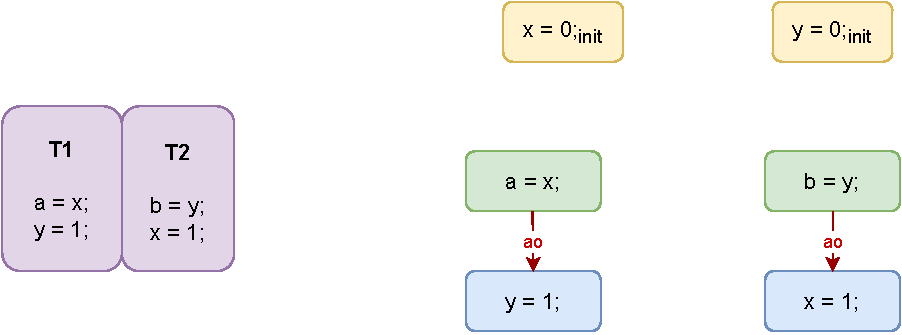
\includegraphics[scale=0.7]{3.ECMAScriptMemoryModel/AgentOrder.pdf}
            \caption{An example with \textit{agent-order} among events.}
            \label{model:agent-order}
        \end{figure}
    
    %Synchronize With Order
    \subsection{Synchronize-With Order ($\stck{_{sw}} $)}
        This is a binary relation between two events that establish synchronization between multiple agents. 
        It is a composition of two sets: 
        \begin{enumerate}
            \item All pairs belonging to $ASW$ of every agent belongs to this ordering relation. 
                \begin{align*}
                    \langle e_i, e_j \rangle \in ASW \Rightarrow{} \reln{e_i}{sw}{e_j}. 
                \end{align*}
                    
            \item Specific reads-from pairs also belong to this ordering relation\footnotemark. 
                \begin{align*}
                    (\reln{r}{rf}{w}) \ \wedge \ \et{r}{sc} \ \wedge \ \et{w}{sc} \ \wedge \ (\Re(r)\!=\!\Re(w)) \ \Rightarrow{} \
                    (\reln{w}{sw}{r}).
                \end{align*}            
        \end{enumerate}
        Figure~\ref{model:sync-with} shows examples of such orders that can exist between events(right) of a program(left).
        The orange box represents the agent-synchronizes-with set that exists coupled with a possible outcome of the program (the final read value of $a$).
        \begin{figure}[H]
            \centering
            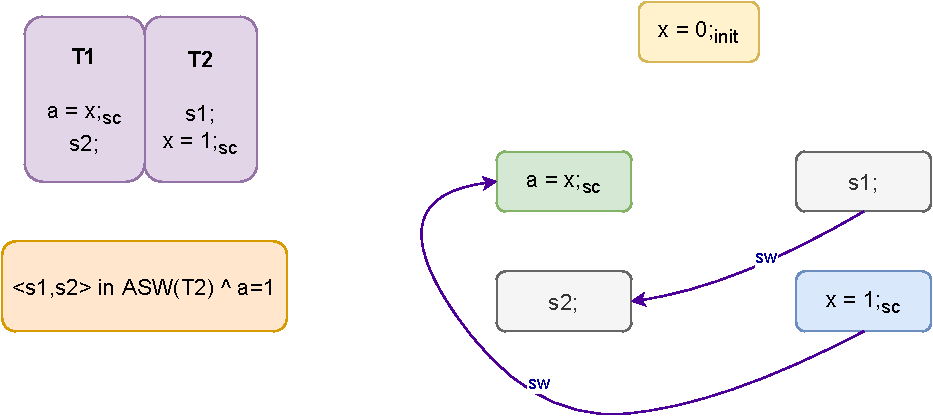
\includegraphics[scale=0.7]{3.ECMAScriptMemoryModel/SynchronizeWith.pdf}
            \caption{An example with \textit{synchronize-with} relations among events.}
            \label{model:sync-with}
        \end{figure}

        \footnotetext{Note that for the second condition, both ranges of events have to be equal. This however, does not mean that the read cannot read from multiple write events(refer the definition for $\stck{_{rbf}}$ in Subsection 3.3).}
        
    %Happens Before order 
    \subsection{Happens Before Order ($\stck{_{hb}}$)}
        This is a transitive order on events, composed of the following:
        \begin{enumerate}
            \item Every agent-ordered relation is also a happens-before relation 
                \begin{align*}
                    (\reln{e}{ao}{d}) \ \Rightarrow{} \ (\reln{e}{hb}{d}).    
                \end{align*}
                
            \item Every synchronize-with relation is also a happens-before relation 
                \begin{align*}
                    (\reln{e}{sw}{d}) \ \Rightarrow{} \ (\reln{e}{hb}{d}).    
                \end{align*}
                 
            \item Initialize type of events happen before all shared memory events that have overlapping or equal ranges between them. 
                \begin{align*}
                    \forall e,d \in SM \ \wedge \ 
                    \et{e}{init} \ \wedge \ 
                    (\Re(e) \cap \Re(d) \neq \phi)
                    \ \Rightarrow{} \ 
                    \reln{e}{hb}{d}.
                \end{align*}          
        \end{enumerate}
        Figure~\ref{model:happens-before} summarizes all possible patterns of happens-before order between events(right) of a program(left).
        THe orange box, again represents the agent-synchronizes-with set that exists coupled with a possible outcome of the program (the final read value of $a$).
        \begin{figure}[H]
            \centering
            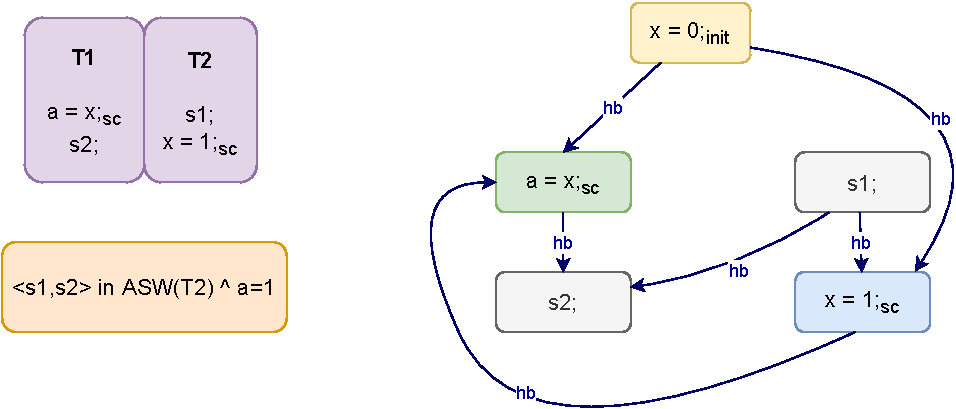
\includegraphics[scale=0.7]{3.ECMAScriptMemoryModel/Happens-before.pdf}
            \caption{An example with all the variants of \textit{happens-before} relations between events.}
            \label{model:happens-before}
        \end{figure}
    
    %Memory Order
    \subsection{Memory Order ($\stck{_{mo}}$)}
        This is a \textit{total order} on all events that respect happens-before order\footnotemark. 
        \begin{align*}
            \reln{e}{hb}{d} \Rightarrow{} \reln{e}{mo}{d}.    
        \end{align*}

        \footnotetext{An interesting part is that memory order, though total, is a bit undefined as to how it weaves together this total order given different events.}
        
        Figure~\ref{model:memory-order} is an example of a memory order between events(right) of a program(left).
        \begin{figure}[H]
            \centering
            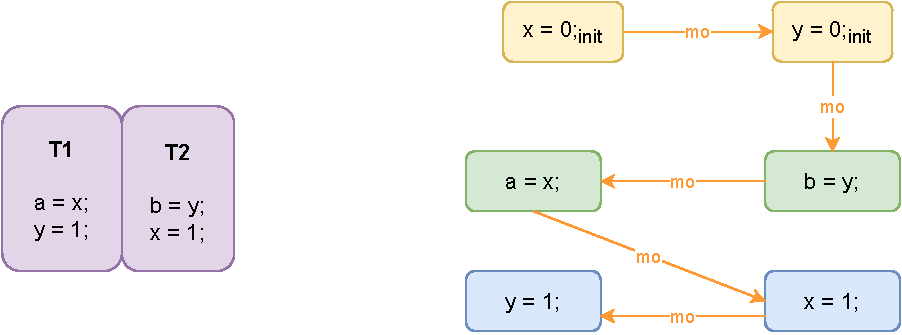
\includegraphics[scale=0.7]{3.ECMAScriptMemoryModel/MemoryOrder.pdf}
            \caption{An example with \textit{memory-order} (total) among all events.}
            \label{model:memory-order}
        \end{figure}
